\title{Computational Neurophysiology - Assignment 1}
\author{Ryan Spangler}
\date{\today}

\documentclass[12pt]{article}

\usepackage{graphicx}

\setcounter{secnumdepth}{0}

\begin{document}
\maketitle

\section{Hypothesis 1}

\emph{Test the hypothesis that the action potential is an "all-or-none" event. i.e. that there is a critical level of stimulus that results in an action potential - below that level no action potential is generated, above that level no further change in the amplitude of the action potential occurs. Draw a graph of maximum membrane potential vs. stimulus amplitude.}

\vspace{10pt}

In the neuron, sodium channels open in response to an increase in voltage, the result of which is to raise the potential, which causes more sodium channels to open in a self-reinforcing cycle.  This sudden influx of sodium and the corresponding rise in potential is what we know as the action potential.  This entire process however requires an initial jolt of current to raise the potential above a point sufficient to trigger this reinforcing cycle, and this level of sufficiency is known as the threshhold.  

If the threshhold hypothesis is correct, there will be a current amplitude below which no action potential occurs, and above which it occurs without fail.  The ultimate level of depolarization should not change much, as if the process is triggered it will continue until all channels are open.  If anything, the lower the amplitude that still triggers the action potential the later the spike will occur, since it will take longer for the self-reinforcing process to gain the necessary momentum to spike.

When run in a series of 20 trials with a stimulus amplitude of 0.0 to 0.4, it shows clearly that the lower the initial amplitude, the longer the spike took to occur.  All spikes that did occur, however, had almost entirely equivalent amplitudes (though did rise slightly).

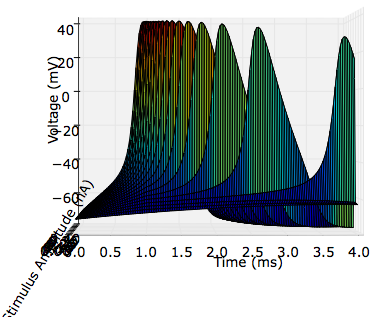
\includegraphics[scale=0.7]{stimulusamp-headon.png}

From another angle it is more clear that the first few trials no action potential is triggered at all.  From 0.0 to about 0.05 nA of initial stimulus current no spike is triggered, where afterwards the spike is triggered without fail, at a progressively sooner time.

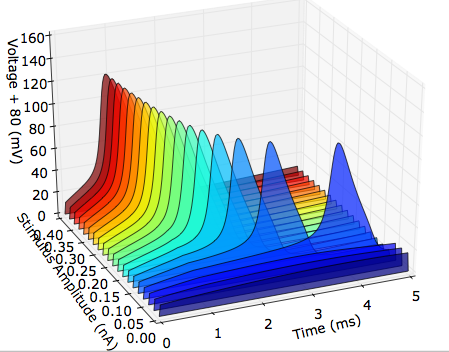
\includegraphics[scale=0.6]{stimulusamp-side.png}

\section{Hypothesis 2}

\emph{Test the hypothesis that the frequency (i.e. number per unit time) of action potentials is determined by the stimulus amplitude.  Draw a graph of the frequency of action potentials vs. the amplitude of the stimulus.}

\section{Hypothesis 3}

\emph{Test the hypothesis that the density of sodium channels determines the rate of rise and amplitude of the action potential.}

\section{Hypothesis 4}

\emph{Test the hypothesis that the density of potassium channels determines the rate at which the action potential falls.  Describe the effect of reducing the Nernst reversal potential for sodium.}

\section{Hypothesis 5}

\emph{Test the hypothesis that the current through the voltage-dependent sodium channels reverses when membrane potential exceeds the Nernst reversal potential for sodium ions.  Describe the dependence of the maximal sodium conductance on the testing level of membrane potential}

\section{Hypothesis 6}

\emph{Test the hypothesis that prior depolarization inactivates voltage-gated sodium channels.}

\section{Hypothesis 7}

\emph{Test the hypothesis that the potassium channels DO NOT inactivate following prior depolarization.}

\end{document} 
